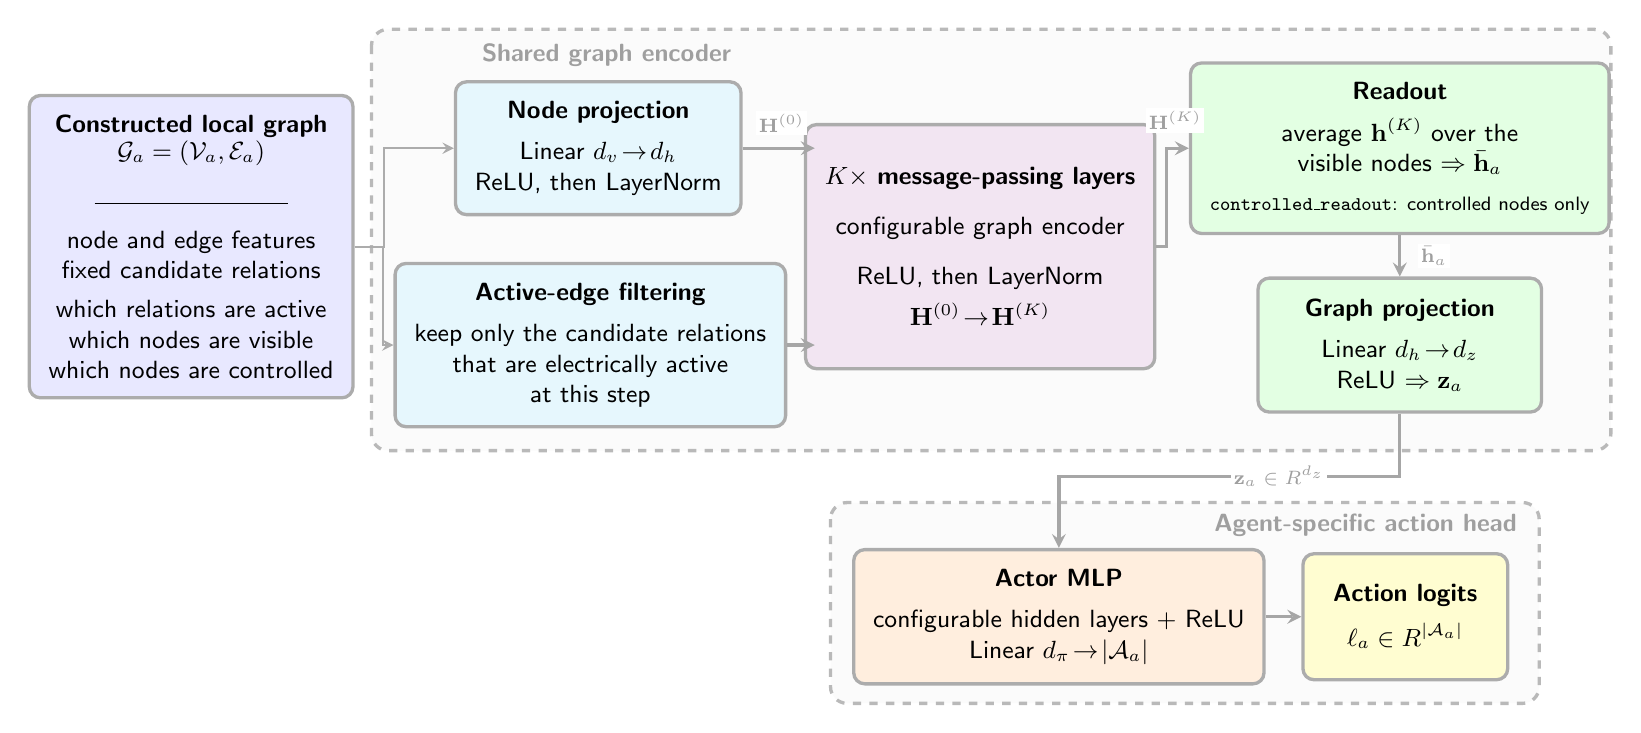
\begin{tikzpicture}[
  >=stealth,
  font=\small\sffamily,
  flow/.style={->, very thick, draw=gray!70},
  branch/.style={->, thick, draw=gray!65},
  stage/.style={
    draw=gray!65,
    very thick,
    rounded corners=4pt,
    align=center,
    text=black,
    inner sep=7pt
  },
  note/.style={font=\scriptsize\sffamily, text=gray!75, fill=white, inner sep=1pt},
  lane/.style={
    draw=gray!55,
    dashed,
    rounded corners=6pt,
    fill=gray!3,
    very thick
  }
]

% Draw.io-style group containers.
\path[lane] (1.12,2.76) rectangle (16.86,-2.59);
\node[anchor=west, font=\bfseries\small\sffamily, text=gray!75]
  at (2.40,2.43) {Shared graph encoder};

\path[lane] (6.95,-3.25) rectangle (15.95,-5.80);
\node[anchor=west, font=\bfseries\small\sffamily, text=gray!75]
  at (11.7,-3.54) {Agent-specific action head};

% Constructed graph.
\node[
  stage,
  fill=blue!9,
  minimum width=3.40cm,
  minimum height=3.45cm
] (graph) at (-1.17,0) {
  {\bfseries Constructed local graph}\\[-1pt]
  $\mathcal{G}_a=(\mathcal{V}_a,\mathcal{E}_a)$\\[5pt]
  \rule{2.45cm}{0.35pt}\\[5pt]
  node and edge features\\
  fixed candidate relations\\[3pt]
  which relations are active\\
  which nodes are visible\\
  which nodes are controlled
};

% Encoder inputs.
\node[
  stage,
  fill=cyan!10,
  minimum width=3.10cm,
  minimum height=1.65cm
] (nodeproj) at (4,1.25) {
  {\bfseries Node projection}\\[4pt]
  Linear $d_v\!\rightarrow\!d_h$\\
  ReLU, then LayerNorm
};

\node[
  stage,
  fill=cyan!10,
  minimum width=3.10cm,
  minimum height=1.65cm
] (filter) at (3.9,-1.25) {
  {\bfseries Active-edge filtering}\\[4pt]
  keep only the candidate relations\\
  that are electrically active\\
  at this step
};

% Repeated message-passing block.
\node[
  stage,
  fill=violet!10,
  minimum width=4.20cm,
  minimum height=3.10cm
] (message) at (8.85,0) {
  {\bfseries $K\times$ message-passing layers}\\[7pt]
  configurable graph encoder\\[7pt]
  ReLU, then LayerNorm\\[4pt]
  $\mathbf{H}^{(0)}\!\rightarrow\!\mathbf{H}^{(K)}$
};

% Readout and shared graph projection.
\node[
  stage,
  fill=green!11,
  minimum width=3.60cm,
  minimum height=1.70cm
] (pool) at (14.18,1.25) {
  {\bfseries Readout}\\[4pt]
  average $\mathbf h^{(K)}$ over the\\
  visible nodes $\Rightarrow\bar{\mathbf h}_a$\\[3pt]
  {\scriptsize \texttt{controlled\_readout}: controlled nodes only}
};

\node[
  stage,
  fill=green!11,
  minimum width=3.60cm,
  minimum height=1.70cm
] (graphproj) at (14.18,-1.25) {
  {\bfseries Graph projection}\\[4pt]
  Linear $d_h\!\rightarrow\!d_z$\\
  ReLU $\Rightarrow \mathbf z_a$
};

% Per-agent policy head and logits.
\node[
  stage,
  fill=orange!13,
  minimum width=4.80cm,
  minimum height=1.60cm
] (actor) at (9.85,-4.7) {
  {\bfseries Actor MLP}\\[4pt]
  configurable hidden layers + ReLU\\
  Linear $d_{\pi}\!\rightarrow\!|\mathcal A_a|$
};

\node[
  stage,
  fill=yellow!18,
  minimum width=2.60cm,
  minimum height=1.60cm
] (logits) at (14.25,-4.7) {
  {\bfseries Action logits}\\[5pt]
  $\boldsymbol{\ell}_a\in
   \mathbb{R}^{|\mathcal A_a|}$
};

% Data flow.
\draw[branch] (graph.east) -- (1.28,0) |- (nodeproj.west);
\draw[branch] (graph.east) -- (1.27,0) |- (filter.west);
\draw[flow] (nodeproj.east) -- node[note, above=4pt, pos=0.54] {$\mathbf H^{(0)}$} (6.75,1.25);
\draw[flow] (filter.east) -- (6.75,-1.25);
\draw[flow] (message.east) -- (11.22,0) |- node[note, above=5pt, pos=0.69] {$\mathbf H^{(K)}$} (pool.west);
\draw[flow] (pool.south) -- node[note, right=6pt] {$\bar{\mathbf h}_a$} (graphproj.north);
\draw[flow] (graphproj.south) -- (14.18,-2.92) -| node[note, near start, right] {$\mathbf z_a\in\mathbb R^{d_z}$} (actor.north);
\draw[flow] (actor.east) -- (logits.west);

\end{tikzpicture}
